%%%%%%%%%%%%%%%%%%%%%%%%%%%%%%%%%%%%%%%%%%%%%%%%%%%%%%%%%%%%%%%%%%%%%%
% Template for a UBC-compliant dissertation
% At the minimum, you will need to change the information found
% after the "Document meta-data"
%
%!TEX TS-program = pdflatex
%!TEX encoding = UTF-8 Unicode

%% The ubcdiss class provides several options:
%%   gpscopy (aka fogscopy)
%%       set parameters to exactly how GPS specifies
%%         * single-sided
%%         * page-numbering starts from title page
%%         * the lists of figures and tables have each entry prefixed
%%           with 'Figure' or 'Table'
%%       This can be tested by `\ifgpscopy ... \else ... \fi'
%%   10pt, 11pt, 12pt
%%       set default font size
%%   oneside, twoside
%%       whether to format for single-sided or double-sided printing
%%   balanced
%%       when double-sided, ensure page content is centred
%%       rather than slightly offset (the default)
%%   singlespacing, onehalfspacing, doublespacing
%%       set default inter-line text spacing; the ubcdiss class
%%       provides \textspacing to revert to this configured spacing
%%   draft
%%       disable more intensive processing, such as including
%%       graphics, etc.
%%

% For submission to GPS
\documentclass[gpscopy,onehalfspacing,11pt]{ubcdiss}

% For your own copies (looks nicer)
% \documentclass[balanced,twoside,11pt]{ubcdiss}

%%%%%%%%%%%%%%%%%%%%%%%%%%%%%%%%%%%%%%%%%%%%%%%%%%%%%%%%%%%%%%%%%%%%%%
%%%%%%%%%%%%%%%%%%%%%%%%%%%%%%%%%%%%%%%%%%%%%%%%%%%%%%%%%%%%%%%%%%%%%%
%%
%% FONTS:
%% 
%% The defaults below configures Times Roman for the serif font,
%% Helvetica for the sans serif font, and Courier for the
%% typewriter-style font.  Configuring fonts can be time
%% consuming; we recommend skipping to END FONTS!
%% 
%% If you're feeling brave, have lots of time, and wish to use one
%% your platform's native fonts, see the commented out bits below for
%% XeTeX/XeLaTeX.  This is not for the faint at heart. 
%% (And shouldn't you be writing? :-)
%%

%% NFSS font specification (New Font Selection Scheme)
\usepackage{times,mathptmx,courier}
\usepackage[scaled=.92]{helvet}

%% Math or theory people may want to include the handy AMS macros
%\usepackage{amssymb}
%\usepackage{amsmath}
%\usepackage{amsfonts}

%% The pifont package provides access to the elements in the dingbat font.   
%% Use \ding{##} for a particular dingbat (see p7 of psnfss2e.pdf)
%%   Useful:
%%     51,52 different forms of a checkmark
%%     54,55,56 different forms of a cross (saltyre)
%%     172-181 are 1-10 in open circle (serif)
%%     182-191 are 1-10 black circle (serif)
%%     192-201 are 1-10 in open circle (sans serif)
%%     202-211 are 1-10 in black circle (sans serif)
%% \begin{dinglist}{##}\item... or dingautolist (which auto-increments)
%% to create a bullet list with the provided character.
\usepackage{pifont}

%%%%%%%%%%%%%%%%%%%%%%%%%%%%%%%%%%%%%%%%%%%%%%%%%%%%%%%%%%%%%%%%%%%%%%
%% Configure fonts for XeTeX / XeLaTeX using the fontspec package.
%% Be sure to check out the fontspec documentation.
%\usepackage{fontspec,xltxtra,xunicode}	% required
%\defaultfontfeatures{Mapping=tex-text}	% recommended
%% Minion Pro and Myriad Pro are shipped with some versions of
%% Adobe Reader.  Adobe representatives have commented that these
%% fonts can be used outside of Adobe Reader.
%\setromanfont[Numbers=OldStyle]{Minion Pro}
%\setsansfont[Numbers=OldStyle,Scale=MatchLowercase]{Myriad Pro}
%\setmonofont[Scale=MatchLowercase]{Andale Mono}

%% Other alternatives:
%\setromanfont[Mapping=tex-text]{Adobe Caslon}
%\setsansfont[Scale=MatchLowercase]{Gill Sans}
%\setsansfont[Scale=MatchLowercase,Mapping=tex-text]{Futura}
%\setmonofont[Scale=MatchLowercase]{Andale Mono}
%\newfontfamily{\SYM}[Scale=0.9]{Zapf Dingbats}
%% END FONTS
%%%%%%%%%%%%%%%%%%%%%%%%%%%%%%%%%%%%%%%%%%%%%%%%%%%%%%%%%%%%%%%%%%%%%%
%%%%%%%%%%%%%%%%%%%%%%%%%%%%%%%%%%%%%%%%%%%%%%%%%%%%%%%%%%%%%%%%%%%%%%



%%%%%%%%%%%%%%%%%%%%%%%%%%%%%%%%%%%%%%%%%%%%%%%%%%%%%%%%%%%%%%%%%%%%%%
%%%%%%%%%%%%%%%%%%%%%%%%%%%%%%%%%%%%%%%%%%%%%%%%%%%%%%%%%%%%%%%%%%%%%%
%%
%% Recommended packages
%%
\usepackage{checkend}	% better error messages on left-open environments
\usepackage{graphicx}	% for incorporating external images

%% booktabs: provides some special commands for typesetting tables as used
%% in excellent journals.  Ignore the examples in the Lamport book!
\usepackage{booktabs}

%% listings: useful support for including source code listings, with
%% optional special keyword formatting.  The \lstset{} causes
%% the text to be typeset in a smaller sans serif font, with
%% proportional spacing.
\usepackage{listings}
\lstset{basicstyle=\sffamily\scriptsize,showstringspaces=false,fontadjust}

%% The acronym package provides support for defining acronyms, providing
%% their expansion when first used, and building glossaries.  See the
%% example in glossary.tex and the example usage throughout the example
%% document.
%% NOTE: to use \MakeTextLowercase in the \acsfont command below,
%%   we *must* use the `nohyperlinks' option -- it causes errors with
%%   hyperref otherwise.  See Section 5.2 in the ``LaTeX 2e for Class
%%   and Package Writers Guide'' (clsguide.pdf) for details.
\usepackage[printonlyused,nohyperlinks]{acronym}

%\usepackage[dvips]{graphicx}
% \usepackage{psfrag}
\usepackage{makeidx} 
\usepackage{amssymb,amsmath,color}
%  \usepackage[hang,small,bf]{caption}
%\usepackage{subfig}
%\usepackage[subfigure]{tocloft}
\usepackage{cite}

\usepackage{algorithmic}
\usepackage{epsfig} 
\usepackage{setspace}
\usepackage{enumerate}
\usepackage{url}
%\usepackage{natbib}
\usepackage[small,compact]{titlesec}
% \usepackage{subfigure}
\newcommand{\refFormula}[1]{(\ref{#1})}
\newcommand{\refFigure}[1]{Figure~\ref{#1}}
% \usepackage{rotating} 

\usepackage{bm}
\usepackage{url,moreverb,graphicx}
\usepackage{ifthen}
\usepackage{amssymb}
\usepackage{listings}
\usepackage{xspace}
\usepackage{rotating}
\usepackage{fixmath}
%\usepackage{relsize}
\usepackage{mdwlist}
%\usepackage{enumitem}
%\usepackage{paralist}
\usepackage{pseudocode}
\usepackage[lined,boxruled]{algorithm2e}
\usepackage{theorem}
\usepackage{amsmath}
\usepackage{multirow}
 \let\labelindent\relax
\usepackage{enumitem}
%\usepackage{floatflt}
%\usepackage{caption}
%\usepackage{natbib}
\usepackage[font=scriptsize]{caption}
\usepackage{setspace}
\usepackage{lipsum}


%\usepackage{subfigure}
\usepackage{balance}

\usepackage{color}
\usepackage{textcomp}
\definecolor{listinggray}{gray}{0.9}
\definecolor{lbcolor}{rgb}{0.9,0.9,0.9}
\lstset{
	%backgroundcolor=\color{lbcolor},
	tabsize=2,
	rulecolor=,
	language=html,
        basicstyle=\scriptsize,
        upquote=true,
        aboveskip={0.5\baselineskip},
        columns=fixed,
        showstringspaces=false,
        extendedchars=true,
        breaklines=true,
        prebreak = \raisebox{0ex}[0ex][0ex]{\ensuremath{\hookleftarrow}},
        frame=single,
        showtabs=false,
        showspaces=false,
        showstringspaces=false,
        identifierstyle=\ttfamily,
        keywordstyle=\color[rgb]{0,0,1},
        commentstyle=\color[rgb]{0.133,0.545,0.133},
        stringstyle=\color[rgb]{0.627,0.126,0.941},
        %emphstyle=\color[rgb]{0.827,0.126,0.941},
}


%Listings for JS
\definecolor{lightgray}{rgb}{.9,.9,.9}
\definecolor{darkgray}{rgb}{.4,.4,.4}
\definecolor{purple}{rgb}{0.65, 0.12, 0.82}
\definecolor{forestgreen}{rgb}{0.13, 0.55, 0.13}

\lstdefinelanguage{JavaScript}{
  keywords={typeof, new, true, false, catch, function, return, null, catch, switch, var, if, for, in, while, do, else, case, break},
  keywordstyle=\color{blue}\bfseries,
  ndkeywords={class, export, boolean, throw, implements, import, this},
  ndkeywordstyle=\color{darkgray}\bfseries,
  identifierstyle=\color{black},
  sensitive=false,
  comment=[l]{//},
  morecomment=[s]{/*}{*/},
  commentstyle=\color{forestgreen}\ttfamily,
  stringstyle=\color{purple}\ttfamily,
  morestring=[b]',
  morestring=[b]"
}
\lstset{
   language=JavaScript,
   %backgroundcolor=\color{lightgray},
   extendedchars=true,
   basicstyle=\scriptsize\ttfamily,
   showstringspaces=false,
   showspaces=false,
   numbers=left,
   numberstyle=\footnotesize,
%   numbersep=-6pt,
   tabsize=1,
   breaklines=true,
   showtabs=false,
   captionpos=b,
   numberblanklines=false,
   escapeinside=\[\]
}

%\textwidth 17.8cm
%\textheight 22.7cm
\setstretch{0.95}

%%Terminology
\newcommand{\rest}{\textsc{Rest}\xspace}
\newcommand{\jsf}{\textsc{Jsf}\xspace}
\newcommand{\ajax}{\textsc{Ajax}\xspace}
\newcommand{\headbf}[1]{\par\smallskip\noindent\textbf{#1.}}
\newcommand{\head}[1]{\subsubsection{#1}}
\newcommand{\headed}[1]{\noindent\textbf{#1}\ \ }
\newcommand{\webtwo}{\textit{Web~2.0}\xspace}
\newcommand{\crawljax}{\textsc{Crawljax}\xspace}
\newcommand{\petstore}{\textsc{PetStore}\xspace}
\newcommand{\etal}{et al.\xspace}
%\newcommand{\ie}{{i.e.,}\xspace}
%\newcommand{\eg}{{e.g.,}\xspace}
\newcommand{\atusatwo}{\textsc{Atusa~2.0}\xspace}
\newcommand{\tudu}{\textsc{TUDU}\xspace}
\newcommand{\todo}{\textsc{Todo}\xspace}
\newcommand{\taskfreak}{\textsc{TaskFreak}\xspace}
\newcommand{\tocview}{\textsc{TocView}\xspace}
\newcommand{\javascript}{{JavaScript}\xspace}
\newcommand{\artemis}{{Artemis}\xspace}
\newcommand{\tool}{{Pythia}\xspace}
\newcommand{\jscover}{{JSCover}\xspace}
\newcommand{\jquery}{\textsc{jQuery}\xspace}
\newcommand{\hitlist}{\textsc{HitList}\xspace}
\newcommand{\googlereader}{\textsc{Google Reader}\xspace}
\newcommand{\testsuite}[1]{\textsc{Test Suite #1}\xspace}
\newcommand{\version}[1]{\textsc{V#1}\xspace}
\newcommand{\proc}[2]{{\textbf{Procedure} \textsc{#1}(\textit{#2})}}
\newcommand{\junit}{\textsc{JUnit}\xspace}
\newcommand{\selenium}{\textsc{Selenium}\xspace}
\newcommand{\qunit}{\textsc{Selenium}\xspace}
\newcommand{\codename}{\textsc{Mutandis}\xspace}
\newcommand{\dustme}{\textsc{DMS}\xspace}
\newcommand{\helium}{\textsc{Helium}\xspace}
\newcommand{\cssess}{\textsc{CSSess}\xspace}
\newcommand{\jsart}{\textsc{JSart}\xspace}


\newcommand{\cssparser}{\textsc{CSSParser}\xspace}

\newcommand{\myspace}{\hspace{1mm}}


%% abbreviations and commands
\newcommand{\secref}[1]{Section~\ref{Sec:#1}}
\newcommand{\figref}[1]{Figure~\ref{Fig:#1}}
\newcommand{\listref}[1]{Listing~\ref{List:#1}}
\newcommand{\tabref}[1]{Table~\ref{Table:#1}}
\newcommand{\algref}[1]{Algorithm~\ref{Alg:#1}}
\newcommand{\curl}[1]{\footnote{~\scriptsize\url{#1}}}
\newcommand{\fn}[1]{\footnote{~\scriptsize{#1}}}
\newcommand{\code}[1]{{\texttt{#1}}}
\newtheorem{mydef}{Definition}


\newcommand{\mycaption}[1]{%
\vspace{-1.3\baselineskip}
\caption{#1}
}

\lstloadlanguages{Java,XML,HTML}



%% The ubcdiss.cls loads the `textcase' package which provides commands
%% for upper-casing and lower-casing text.  The following causes
%% the acronym package to typeset acronyms in small-caps
%% as recommended by Bringhurst.


\renewcommand{\acsfont}[1]{{\scshape \MakeTextLowercase{#1}}}

%% color: add support for expressing colour models.  Grey can be used
%% to great effect to emphasize other parts of a graphic or text.
%% For an excellent set of examples, see Tufte's "Visual Display of
%% Quantitative Information" or "Envisioning Information".
\usepackage{color}
\definecolor{greytext}{gray}{0.5}

%% comment: provides a new {comment} environment: all text inside the
%% environment is ignored.
%%   \begin{comment} ignored text ... \end{comment}
\usepackage{comment}

%% The natbib package provides more sophisticated citing commands
%% such as \citeauthor{} to provide the author names of a work,
%% \citet{} to produce an author-and-reference citation,
%% \citep{} to produce a parenthetical citation.
%% We use \citeeg{} to provide examples
\usepackage[numbers,sort&compress]{natbib}
\newcommand{\citeeg}[1]{\citep[e.g.,][]{#1}}

%% The titlesec package provides commands to vary how chapter and
%% section titles are typeset.  The following uses more compact
%% spacings above and below the title.  The titleformat that follow
%% ensure chapter/section titles are set in singlespace.
\usepackage[compact]{titlesec}
\titleformat*{\section}{\singlespacing\raggedright\bfseries\Large}
\titleformat*{\subsection}{\singlespacing\raggedright\bfseries\large}
\titleformat*{\subsubsection}{\singlespacing\raggedright\bfseries}
\titleformat*{\paragraph}{\singlespacing\raggedright\itshape}

%% The caption package provides support for varying how table and
%% figure captions are typeset.
\usepackage[format=hang,indention=-1cm,labelfont={bf},margin=1em]{caption}

%% url: for typesetting URLs and smart(er) hyphenation.
%% \url{http://...} 
\usepackage{url}
\urlstyle{sf}	% typeset urls in sans-serif


%%%%%%%%%%%%%%%%%%%%%%%%%%%%%%%%%%%%%%%%%%%%%%%%%%%%%%%%%%%%%%%%%%%%%%
%%%%%%%%%%%%%%%%%%%%%%%%%%%%%%%%%%%%%%%%%%%%%%%%%%%%%%%%%%%%%%%%%%%%%%
%%
%% Possibly useful packages: you may need to explicitly install
%% these from CTAN if they aren't part of your distribution;
%% teTeX seems to ship with a smaller base than MikTeX and MacTeX.
%%
%\usepackage{pdfpages}	% insert pages from other PDF files
%\usepackage{longtable}	% provide tables spanning multiple pages
%\usepackage{chngpage}	% support changing the page widths on demand
%\usepackage{tabularx}	% an enhanced tabular environment

%% enumitem: support pausing and resuming enumerate environments.
%\usepackage{enumitem}

%% rotating: provides two environments, sidewaystable and sidewaysfigure,
%% for typesetting tables and figures in landscape mode.  
%\usepackage{rotating}

%% subfig: provides for including subfigures within a figure,
%% and includes being able to separately reference the subfigures.
%\usepackage{subfig}

%% ragged2e: provides several new new commands \Centering, \RaggedLeft,
%% \RaggedRight and \justifying and new environments Center, FlushLeft,
%% FlushRight and justify, which set ragged text and are easily
%% configurable to allow hyphenation.
%\usepackage{ragged2e}

%% The ulem package provides a \sout{} for striking out text and
%% \xout for crossing out text.  The normalem and normalbf are
%% necessary as the package messes with the emphasis and bold fonts
%% otherwise.
%\usepackage[normalem,normalbf]{ulem}    % for \sout

%%%%%%%%%%%%%%%%%%%%%%%%%%%%%%%%%%%%%%%%%%%%%%%%%%%%%%%%%%%%%%%%%%%%%%
%% HYPERREF:
%% The hyperref package provides for embedding hyperlinks into your
%% document.  By default the table of contents, references, citations,
%% and footnotes are hyperlinked.
%%
%% Hyperref provides a very handy command for doing cross-references:
%% \autoref{}.  This is similar to \ref{} and \pageref{} except that
%% it automagically puts in the *type* of reference.  For example,
%% referencing a figure's label will put the text `Figure 3.4'.
%% And the text will be hyperlinked to the appropriate place in the
%% document.
%%
%% Generally hyperref should appear after most other packages

%% The following puts hyperlinks in very faint grey boxes.
%% The `pagebackref' causes the references in the bibliography to have
%% back-references to the citing page; `backref' puts the citing section
%% number.  See further below for other examples of using hyperref.
%% 2009/12/09: now use `linktocpage' (Jacek Kisynski): GPS now prefers
%%   that the ToC, LoF, LoT place the hyperlink on the page number,
%%   rather than the entry text.
\usepackage[bookmarks,bookmarksnumbered,%
    allbordercolors={0.8 0.8 0.8},%
    pagebackref,linktocpage%
    ]{hyperref}
%% The following change how the the back-references text is typeset in a
%% bibliography when `backref' or `pagebackref' are used
\renewcommand\backrefpagesname{\(\rightarrow\) pages}
\renewcommand\backref{\textcolor{greytext} \backrefpagesname\ }

%% The following uses most defaults, which causes hyperlinks to be
%% surrounded by colourful boxes; the colours are only visible in
%% PDFs and don't show up when printed:
%\usepackage[bookmarks,bookmarksnumbered]{hyperref}

%% The following disables the colourful boxes around hyperlinks.
%\usepackage[bookmarks,bookmarksnumbered,pdfborder={0 0 0}]{hyperref}

%% The following disables all hyperlinking, but still enabled use of
%% \autoref{}
%\usepackage[draft]{hyperref}

%% The following commands causes chapter and section references to
%% uppercase the part name.
\renewcommand{\chapterautorefname}{Chapter}
\renewcommand{\sectionautorefname}{Section}
\renewcommand{\subsectionautorefname}{Section}
\renewcommand{\subsubsectionautorefname}{Section}

%% If you have long page numbers (e.g., roman numbers in the 
%% preliminary pages for page 28 = xxviii), you might need to
%% uncomment the following and tweak the \@pnumwidth length
%% (default: 1.55em).  See the tocloft documentation at
%% http://www.ctan.org/tex-archive/macros/latex/contrib/tocloft/
% \makeatletter
% \renewcommand{\@pnumwidth}{3em}
% \makeatother

%%%%%%%%%%%%%%%%%%%%%%%%%%%%%%%%%%%%%%%%%%%%%%%%%%%%%%%%%%%%%%%%%%%%%%
%%%%%%%%%%%%%%%%%%%%%%%%%%%%%%%%%%%%%%%%%%%%%%%%%%%%%%%%%%%%%%%%%%%%%%
%%
%% Some special settings that controls how text is typeset
%%
% \raggedbottom		% pages don't have to line up nicely on the last line
% \sloppy		% be a bit more relaxed in inter-word spacing
% \clubpenalty=10000	% try harder to avoid orphans
% \widowpenalty=10000	% try harder to avoid widows
% \tolerance=1000

%% And include some of our own useful macros
% This file provides examples of some useful macros for typesetting
% dissertations.  None of the macros defined here are necessary beyond
% for the template documentation, so feel free to change, remove, and add
% your own definitions.
%
% We recommend that you define macros to separate the semantics
% of the things you write from how they are presented.  For example,
% you'll see definitions below for a macro \file{}: by using
% \file{} consistently in the text, we can change how filenames
% are typeset simply by changing the definition of \file{} in
% this file.
% 
%% The following is a directive for TeXShop to indicate the main file
%%!TEX root = diss.tex

\newcommand{\NA}{\textsc{n/a}}	% for "not applicable"
\newcommand{\eg}{e.g.,\ }	% proper form of examples (\eg a, b, c)
\newcommand{\ie}{i.e.,\ }	% proper form for that is (\ie a, b, c)
%\newcommand{\etal}{\emph{et al}}

% Some useful macros for typesetting terms.
\newcommand{\file}[1]{\texttt{#1}}
\newcommand{\class}[1]{\texttt{#1}}
\newcommand{\latexpackage}[1]{\href{http://www.ctan.org/macros/latex/contrib/#1}{\texttt{#1}}}
\newcommand{\latexmiscpackage}[1]{\href{http://www.ctan.org/macros/latex/contrib/misc/#1.sty}{\texttt{#1}}}
\newcommand{\env}[1]{\texttt{#1}}
\newcommand{\BibTeX}{Bib\TeX}

% Define a command \doi{} to typeset a digital object identifier (DOI).
% Note: if the following definition raise an error, then you likely
% have an ancient version of url.sty.  Either find a more recent version
% (3.1 or later work fine) and simply copy it into this directory,  or
% comment out the following two lines and uncomment the third.
\DeclareUrlCommand\DOI{}
\newcommand{\doi}[1]{\href{http://dx.doi.org/#1}{\DOI{doi:#1}}}
%\newcommand{\doi}[1]{\href{http://dx.doi.org/#1}{doi:#1}}

% Useful macro to reference an online document with a hyperlink
% as well with the URL explicitly listed in a footnote
% #1: the URL
% #2: the anchoring text
\newcommand{\webref}[2]{\href{#1}{#2}\footnote{\url{#1}}}

% epigraph is a nice environment for typesetting quotations
\makeatletter
\newenvironment{epigraph}{%
	\begin{flushright}
	\begin{minipage}{\columnwidth-0.75in}
	\begin{flushright}
	\@ifundefined{singlespacing}{}{\singlespacing}%
    }{
	\end{flushright}
	\end{minipage}
	\end{flushright}}
\makeatother

% \FIXME{} is a useful macro for noting things needing to be changed.
% The following definition will also output a warning to the console
\newcommand{\FIXME}[1]{\typeout{**FIXME** #1}\textbf{[FIXME: #1]}}

% END


%%%%%%%%%%%%%%%%%%%%%%%%%%%%%%%%%%%%%%%%%%%%%%%%%%%%%%%%%%%%%%%%%%%%%%
%%%%%%%%%%%%%%%%%%%%%%%%%%%%%%%%%%%%%%%%%%%%%%%%%%%%%%%%%%%%%%%%%%%%%%
%%
%% Document meta-data: be sure to also change the \hypersetup information
%%

\title{Effective Test Generation and Adequacy Assessment for JavaScript-based Web Applications}
%\subtitle{If you want a subtitle}

\author{Shabnam Mirshokraie}
\previousdegree{BSc. Computer Engineering,  Ferdowsi University of Mashhad, Iran, 2006}
\previousdegree{MSc. Computing Science, Simon Fraser University, Canada, 2010}

% What is this dissertation for?
\degreetitle{Doctor of Philosophy}

\institution{The University of British Columbia}
\campus{Vancouver}

\faculty{The Faculty of Applied Science}
\department{Electrical and Computer Engineering}
\submissionmonth{April}
\submissionyear{2015}

%% hyperref package provides support for embedding meta-data in .PDF
%% files
\hypersetup{
  pdftitle={Change this title!  (DRAFT: \today)},
  pdfauthor={Johnny Canuck},
  pdfkeywords={Your keywords here}
}

%%%%%%%%%%%%%%%%%%%%%%%%%%%%%%%%%%%%%%%%%%%%%%%%%%%%%%%%%%%%%%%%%%%%%%
%%%%%%%%%%%%%%%%%%%%%%%%%%%%%%%%%%%%%%%%%%%%%%%%%%%%%%%%%%%%%%%%%%%%%%
%% 
%% The document content
%%

%% LaTeX's \includeonly commands causes any uses of \include{} to only
%% include files that are in the list.  This is helpful to produce
%% subsets of your thesis (e.g., for committee members who want to see
%% the dissertation chapter by chapter).  It also saves time by 
%% avoiding reprocessing the entire file.
%\includeonly{intro,conclusions}
%\includeonly{discussion}

\begin{document}

%%%%%%%%%%%%%%%%%%%%%%%%%%%%%%%%%%%%%%%%%%%%%%%%%%
%% From Thesis Components: Tradtional Thesis
%% <http://www.grad.ubc.ca/current-students/dissertation-thesis-preparation/order-components>

% Preliminary Pages (numbered in lower case Roman numerals)
%    1. Title page (mandatory)
\maketitle

%    2. Abstract (mandatory - maximum 350 words)
\begin{abstract}
% MUST be 150 words or less
%Developers often test their web applications using frameworks such as Selenium. Although such frameworks help to automate test execution, the test cases need to be written manually, which is tedious and inefficient.
The event-driven and highly dynamic nature of \javascript, as well as its runtime interaction with the Document Object Model (DOM) make it  challenging to test \javascript applications.
Although current web test automation techniques target the generation of event sequences, they ignore testing the \javascript code at the unit level. Further they either ignore the oracle problem completely or simplify it through generic soft oracles such as HTML validation and runtime exceptions. We present a framework to automatically generate
 test cases for \javascript applications at two complementary levels, namely events and individual \javascript  
functions. In addition, these test cases are strengthened by automatically generated mutation-based oracles. % capable of detecting regression faults in \javascript code and the DOM. 
Our approach employs a combination of function converge maximization and function state abstraction algorithms to efficiently generate unit test cases.
We empirically evaluate the implementation of our approach, called \tool, to assess its efficacy. 
The results, on 13 \javascript-based applications, show that the generated test cases achieve a coverage of 68\% and that \tool can detect injected \javascript and DOM faults with a high accuracy (100\% precision, 70\% recall).
We also find that \tool outperforms an existing \javascript test automation framework both in terms of coverage and detected faults.
%Testing JavaScript-based applications is challenging as manually exploring various execution paths of the application is difficult.
%Also JavaScript's highly dynamic nature as well as its complex interaction with the DOM make it difficult for the tester to achieve high coverage. 

%In current practice of \javascript testing, developers often write test cases manually using unit testing frameworks such as Selenium. While such tools help testers to design a test suite by providing an environment to record GUI actions, \javascript testing still remains a challenging task as manually exploring various execution paths of the application is difficult. Even after detecting an incorrect behaviour of the application, \javascript's highly dynamic nature as well as its complex interaction with Document Object Model (DOM) make it difficult for the tester to achieve high coverage. In this paper, we present a framework to automatically generate unit tests for web applications at two levels: (1) individual \javascript functions, (2) DOM event sequences. These  test cases are strengthened by automatically generated mutation-based oracles capable of detecting faults in \javascript code as well as the DOM tree. We implement our approach in a tool called \tool. We empirically evaluate \tool, by comparing it to another existing \javascript test generator, to assess its efficacy in terms of achieved coverage by the generated test suite as well as fault finding capability.
\end{abstract}
\cleardoublepage

%    3. Preface
%% The following is a directive for TeXShop to indicate the main file
%%!TEX root = diss.tex

\chapter{Preface}
During my PhD studies, I have conducted the research described in this dissertation in collaboration with my supervisors, Ali Mesbah and Karthik Pattabiraman at the University of British Columbia (UBC). 
Research projects included in this dissertation have been either published or currently under review. I was the main contributor for the research projects presented in each chapter, including the initial idea, developing, and evaluating the system. I had the collaboration of Ali Mesbah and Karthik Pattabiraman to discuss the projects and ideas, as well as making edits in the text. 

The following list presents publications for each chapter.
\begin{itemize}
\item \chapref{jsart}:
\begin{itemize}
\item ``\jsart: JavaScript Assertion-based Regression Testing" \cite{mirshokraie:icwe12},
S. Mirshokraie and A. Mesbah, International Conferencee on Web Engineering (ICWE), 2012, 238-252.
\end{itemize}
\item \chapref{mutandis}:
\begin{itemize}
\item ``Efficient JavaScript Mutation Testing" \cite{mirshokraie:icst13},
S. Mirshokraie, A. Mesbah and K. Pattabiraman, International Conference on Software Testing, Verification, and Validation (ICST), 2013, 74-83 (Best paper Runner-up award).
\item ``Guided Mutation Testing for JavaScript Web Applications" \cite{mirshokraie:tse15},
S. Mirshokraie, A. Mesbah and K. Pattabiraman, IEEE Transaction on Software Engineering (TSE), 2015, 429-444.
\end{itemize}
\item \chapref{jseft}:
\begin{itemize}
\item ``JSEFT: Automated JavaScript Unit Test Generation" \cite{mirshokraie:icst15},
S. Mirshokraie, A. Mesbah and K. Pattabiraman, International Conference on Software Testing, Verification, and Validation (ICST), 2015, 1-10 (Nominated for the best paper award).
\item ``PY\-THIA: Generating Test Cases with Oracles
for JavaScript Applications" \cite{shabnam:ase13},
S. Mirshokraie, A. Mesbah and K. Pattabiraman, Automated Software Engineering (ASE), 2013, New Ideas Track, 610-615.
%\item ``Unit Test Generation for JavaScript", S. Mirshokraie, A. Mesbah and K. Pattabiraman,
%Submitted to the Software Testing, Verification and Reliability (STVR) journal and is currently under review. 
\end{itemize} 
%\item \chapref{atrina}:
%\begin{itemize}
%\item ``Atrina: Inferring Unit Oracles from GUI Test Cases",
%Submitted to the International Conference on Software Testing, Verification, and Validation (ICST'16) and is currently under review.
%\end{itemize}
\end{itemize}

%At \ac{UBC}, a preface may be required.  Be sure to check the
%\ac{GPS} guidelines as they may have specific content to be included.

\cleardoublepage

%    4. Table of contents (mandatory - list all items in the preliminary pages
%    starting with the abstract, followed by chapter headings and
%    subheadings, bibliographies and appendices)
\tableofcontents
\cleardoublepage	% required by tocloft package

%    5. List of tables (mandatory if thesis has tables)
\listoftables
\cleardoublepage	% required by tocloft package

%    6. List of figures (mandatory if thesis has figures)
\listoffigures
\cleardoublepage	% required by tocloft package

%    7. List of illustrations (mandatory if thesis has illustrations)
%    8. Lists of symbols, abbreviations or other (optional)

%    9. Glossary (optional)
%%% The following is a directive for TeXShop to indicate the main file
%%!TEX root = diss.tex

\chapter{Glossary}

This glossary uses the handy \latexpackage{acroynym} package to automatically
maintain the glossary.  It uses the package's \texttt{printonlyused}
option to include only those acronyms explicitly referenced in the
\LaTeX\ source.

% use \acrodef to define an acronym, but no listing
\acrodef{UI}{user interface}
\acrodef{UBC}{University of British Columbia}

% The acronym environment will typeset only those acronyms that were
% *actually used* in the course of the document
\begin{acronym}[ANOVA]
\acro{ANOVA}[ANOVA]{Analysis of Variance\acroextra{, a set of
  statistical techniques to identify sources of variability between groups}}
\acro{API}{application programming interface}
\acro{CTAN}{\acroextra{The }Common \TeX\ Archive Network}
\acro{DOI}{Document Object Identifier\acroextra{ (see
    \url{http://doi.org})}}
\acro{GPS}[GPS]{Graduate and Postdoctoral Studies}
\acro{PDF}{Portable Document Format}
\acro{RCS}[RCS]{Revision control system\acroextra{, a software
    tool for tracking changes to a set of files}}
\acro{TLX}[TLX]{Task Load Index\acroextra{, an instrument for gauging
  the subjective mental workload experienced by a human in performing
  a task}}
\acro{UML}{Unified Modelling Language\acroextra{, a visual language
    for modelling the structure of software artefacts}}
\acro{URL}{Unique Resource Locator\acroextra{, used to describe a
    means for obtaining some resource on the world wide web}}
\acro{W3C}[W3C]{\acroextra{the }World Wide Web Consortium\acroextra{,
    the standards body for web technologies}}
\acro{XML}{Extensible Markup Language}
\end{acronym}

% You can also use \newacro{}{} to only define acronyms
% but without explictly creating a glossary
% 
% \newacro{ANOVA}[ANOVA]{Analysis of Variance\acroextra{, a set of
%   statistical techniques to identify sources of variability between groups.}}
% \newacro{API}[API]{application programming interface}
% \newacro{GOMS}[GOMS]{Goals, Operators, Methods, and Selection\acroextra{,
%   a framework for usability analysis.}}
% \newacro{TLX}[TLX]{Task Load Index\acroextra{, an instrument for gauging
%   the subjective mental workload experienced by a human in performing
%   a task.}}
% \newacro{UI}[UI]{user interface}
% \newacro{UML}[UML]{Unified Modelling Language}
% \newacro{W3C}[W3C]{World Wide Web Consortium}
% \newacro{XML}[XML]{Extensible Markup Language}
	% always input, since other macros may rely on it

\textspacing		% begin one-half or double spacing

%   10. Acknowledgements (optional)
%% The following is a directive for TeXShop to indicate the main file
%%!TEX root = diss.tex

\chapter{Acknowledgments}
I would like to express my deepest gratitude to my senior supervisor, Ali Mesbah,
for mentoring me in the past four years with his patience and knowledge. Without his support, completion of this thesis would not have been possible for me.
I would also like to express my gratitude to Karthik Pattabiraman for the enriching feedback he provided during the conversations we had. The knowledge that I have gained through the insightful
discussions with Karthik are invaluable.

I am grateful to all the members at the Software Analysis and Testing Lab for providing me a stimulating and fun environment. Last but certainly not least, I owe my deepest gratitude to my
parents for their love and endless support. I will never forget what I owe them, and my eternal gratitude to them cannot be expressed by words. I deeply appreciate the never-ending patience I have received from my parents.




%   11. Dedication (optional)

% Body of Thesis (not all sections may apply)
\mainmatter

\acresetall	% reset all acronyms used so far

%    1. Introduction
\section{Introduction} \label{Sec:intro}

\javascript has emerged as the lingua franca of modern, interactive web applications. 
The interactivity is made possible by the close relation between the Document Object Model (DOM) and the underlying \javascript code.
However, testing modern web applications is challenging.  
To check the application's behaviour from an end-user's perspective, testers often use popular frameworks such as Selenium. 
The main advantage of using these frameworks to write DOM-based tests and assertions is that they require little knowledge about the internal operations performed by the code. 
Rather, the tester needs only basic knowledge of common event sequences to cover important DOM elements to assert. 
%This makes it easier for the tester to write DOM-based test suites.

 
On the other hand, it is more tedious to
write unit test assertions for web applications that have rich interaction with the DOM through their \javascript code. 
This is because the tester needs to precisely understand the full range of interaction between the code level operations of a unit and the DOM level operations of a system, 
and thus may fail to assert the correctness of a particular behaviour when the unit is used as a part of a system. 
Our previous findings \cite{mirshokraie:icst15} indicate that while DOM-based assertions tend to miss the related portion of
code-level failure, more fine grained unit-level assertions can detect such faults. 
Furthermore, finding the root cause of an error during DOM-based testing is much more expensive than during unit testing.
This suggest that we need unit-level tests to complement existing DOM-based test for more effective fault detection and localization.
%The inherent characteristics of unit and DOM-based tests, indicate that they are complementary and that there is a trade-off in individually using each to detect faults. 

Current test generation approaches either produce unit test oracles based on mutation testing techniques \cite{mirshokraie:icst15, fraser:tse12}, or rely on soft oracles \cite{artzi:icse11}. Mutation-based approaches suffer from high computational cost, and the problem of equivalent mutants (which are syntactically different but semantically the same as the original application).
Soft oracles such as HTML validation and runtime exceptions are also limited in that they fail to capture logical and computational errors. 
Recently, Milani Fard \etal \cite{milanifard:ase14} proposed using the DOM-based test suite of a web application to regenerate assertions for newly detected states through exploring alternative paths of the application. However, the new assertions generated by this technique remain at the DOM-level without considering the relation between the \javascript code and the DOM.
In this work, we propose to exploit an existing DOM-based test suite to generate unit-level assertions at the code-level for applications that interact highly with the DOM through the underlying \javascript code. We utilize
existing DOM-dependent assertions as well as useful execution information inferred from a DOM-based test suite to automatically generate assertions used for testing individual \javascript functions. 
{\em To the best of our knowledge, this work is the first to propose an approach for generating unit-level assertions by using existing DOM-based test suites.} 

The main contributions of our work include:
\begin{itemize}[noitemsep]
\item A slicing-based technique to generate unit-level assertions for testing JavaScr\-ipt functions by utilizing existing DOM-based test assertions;
\item A technique for selectively choosing additional DOM elements to assert on that are unchecked in the existing DOM-based test suite;
\item An implementation of our approach in a tool, called \atrina; 
\item An empirical evaluation to assess the efficacy of the approach on seven open-source web applications;
The results show that the assertions generated by \atrina surpass the fault finding capabilities of (1) the human-written DOM-based assertions by 31\% on average, and (2) the state-of-the-art mutation-based assertion generation technique by 26\% on average.
\end{itemize} 

%    2. Main body
% Generally recommended to put each chapter into a separate file
%\include{relatedwork}
%\include{model}
%\include{impl}
%\subsection{Discussion} \label{Sec:discussion}
\begin{figure}[!t]
  \centering
  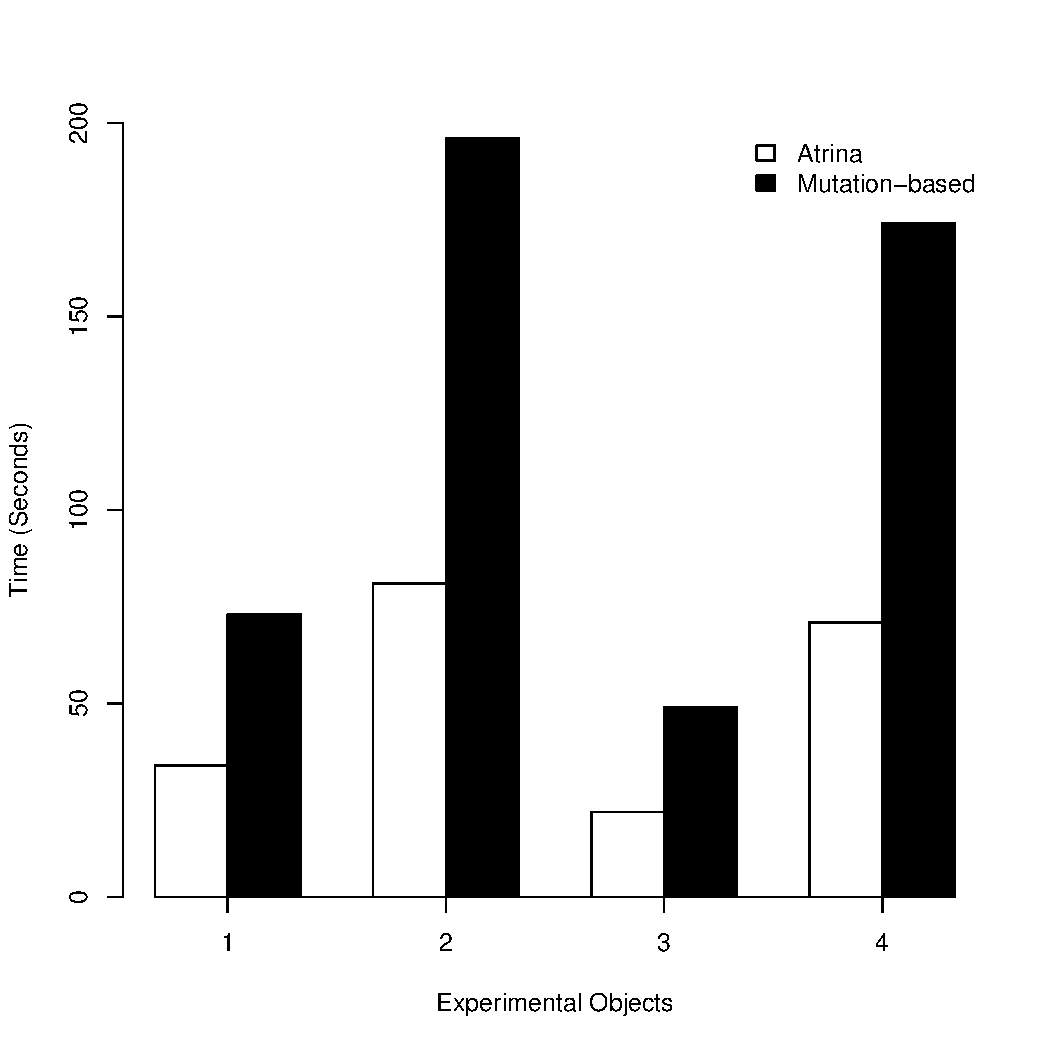
\includegraphics[width=0.7\hsize]{r-scripts/performance}
  \vspace{-0.18in}   
  \mycaption{Time overhead for each approach.}
  \vspace{-0.3in} 
  \label{Fig:performance}   
\end{figure}
% Moved time efficiency to results
%Moreover, this reiterates the known performance shortcomings of approaches that rely on mutant generation.
\headbf{Fault Masking} As we mentioned in \secref{explicitAssertions}, the concrete value of an entity in the computed backward slice can potentially be used as the expected value of the entity in explicit assertions to test the current version of the application.
The actual values of the related entities in the backward slice are correct unless there exists a masked fault which is concealed in the chain of computations and thus does not propagate to the checked state of the DOM element. However, we conjecture that fault masking rarely happens in \javascript web applications as it is more prevalent in programs with many small expressions whose results are stored in several intermediate values. We also observed no fault masking occurrence during the evaluation of \tool on seven \javascript applications used in this study.
\headbf{Limitations} The effectiveness of the generated assertions by \tool in terms of fault finding capability depends on the quality of human-written DOM-based test cases. If the DOM assertions contained in the DOM-based test suite check irrelevant information, the explicit assertions obtained by our tool will point to entities that may not be important from the tester's point of view. This can also negatively affect the fault finding capability of implicit assertions as they are indirectly inferred from the DOM-based assertions. Moreover, if the human-written test suite does not execute application's state with effective DOM elements, our tool is not able to infer effective candidate assertions.   
%\include{conclusions}

%    3. Notes
%    4. Footnotes

%    5. Bibliography
\begin{singlespace}
\raggedright
\bibliographystyle{abbrvnat}
\bibliography{../biblio}
\end{singlespace}

\appendix
%    6. Appendices (including copies of all required UBC Research
%       Ethics Board's Certificates of Approval)
%\include{reb-coa}	% pdfpages is useful here
\chapter{Supporting Materials}

This would be any supporting material not central to the dissertation.
For example:
\begin{itemize}
\item additional details of methodology and/or data;
\item diagrams of specialized equipment developed.;
\item copies of questionnaires and survey instruments.
\end{itemize}


\backmatter
%    7. Index
% See the makeindex package: the following page provides a quick overview
% <http://www.image.ufl.edu/help/latex/latex_indexes.shtml>


\end{document}
